    \chapter{Methodology}
       \section{SOFTWARE DEVELOPMENT APPROACH}
        Prototyping model is a type of software develpoment model. It is an iterative approach where a basic prototype is constructed to gain a better understanding of the project. This prototype is typically incomplete or lacking many components. The model is then refined based on feedback and system is reconstructed iteratively until desired conditions are met.
         \begin{figure}[hbt!]
            \center{
                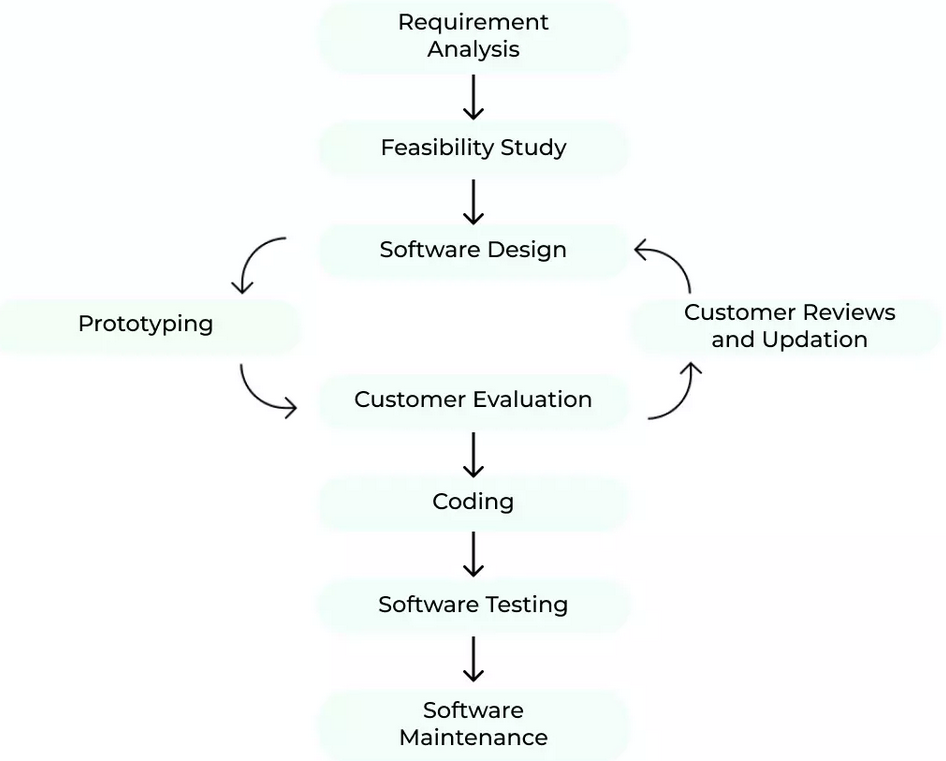
\includegraphics[width=0.75\textwidth]{./img/prototype model.png}
                \caption{Prototype Model for Software Development}
            }
        \end{figure}
        \section{DATA COLLECTION}
        We have decided to use the dataset that consists of 70k REAL faces from the Flickr dataset collected by Nvidia, as well as 70k fake faces sampled from the 1 Million FAKE faces (generated by StyleGAN) that was provided by Bojan which was compiled by xhlulu on kaggle.\\
        \url{https://www.kaggle.com/datasets/xhlulu/140k-real-and-fake-faces}
    
        \section{Implementation}
        Deepfake images are structured and classified into fake and real face. The dataset generated is splited into 80\% training set and 20\% test set. The training set is then fed into a Deep learning model (ResNet Architecture) which is repeatedly tested and iterated to generate a model that can predict the deepfake images. The model is tested using test set to generate evaluation metrics.
        \vspace{0.5in}
        \begin{figure}[hbt!]
            \center{
                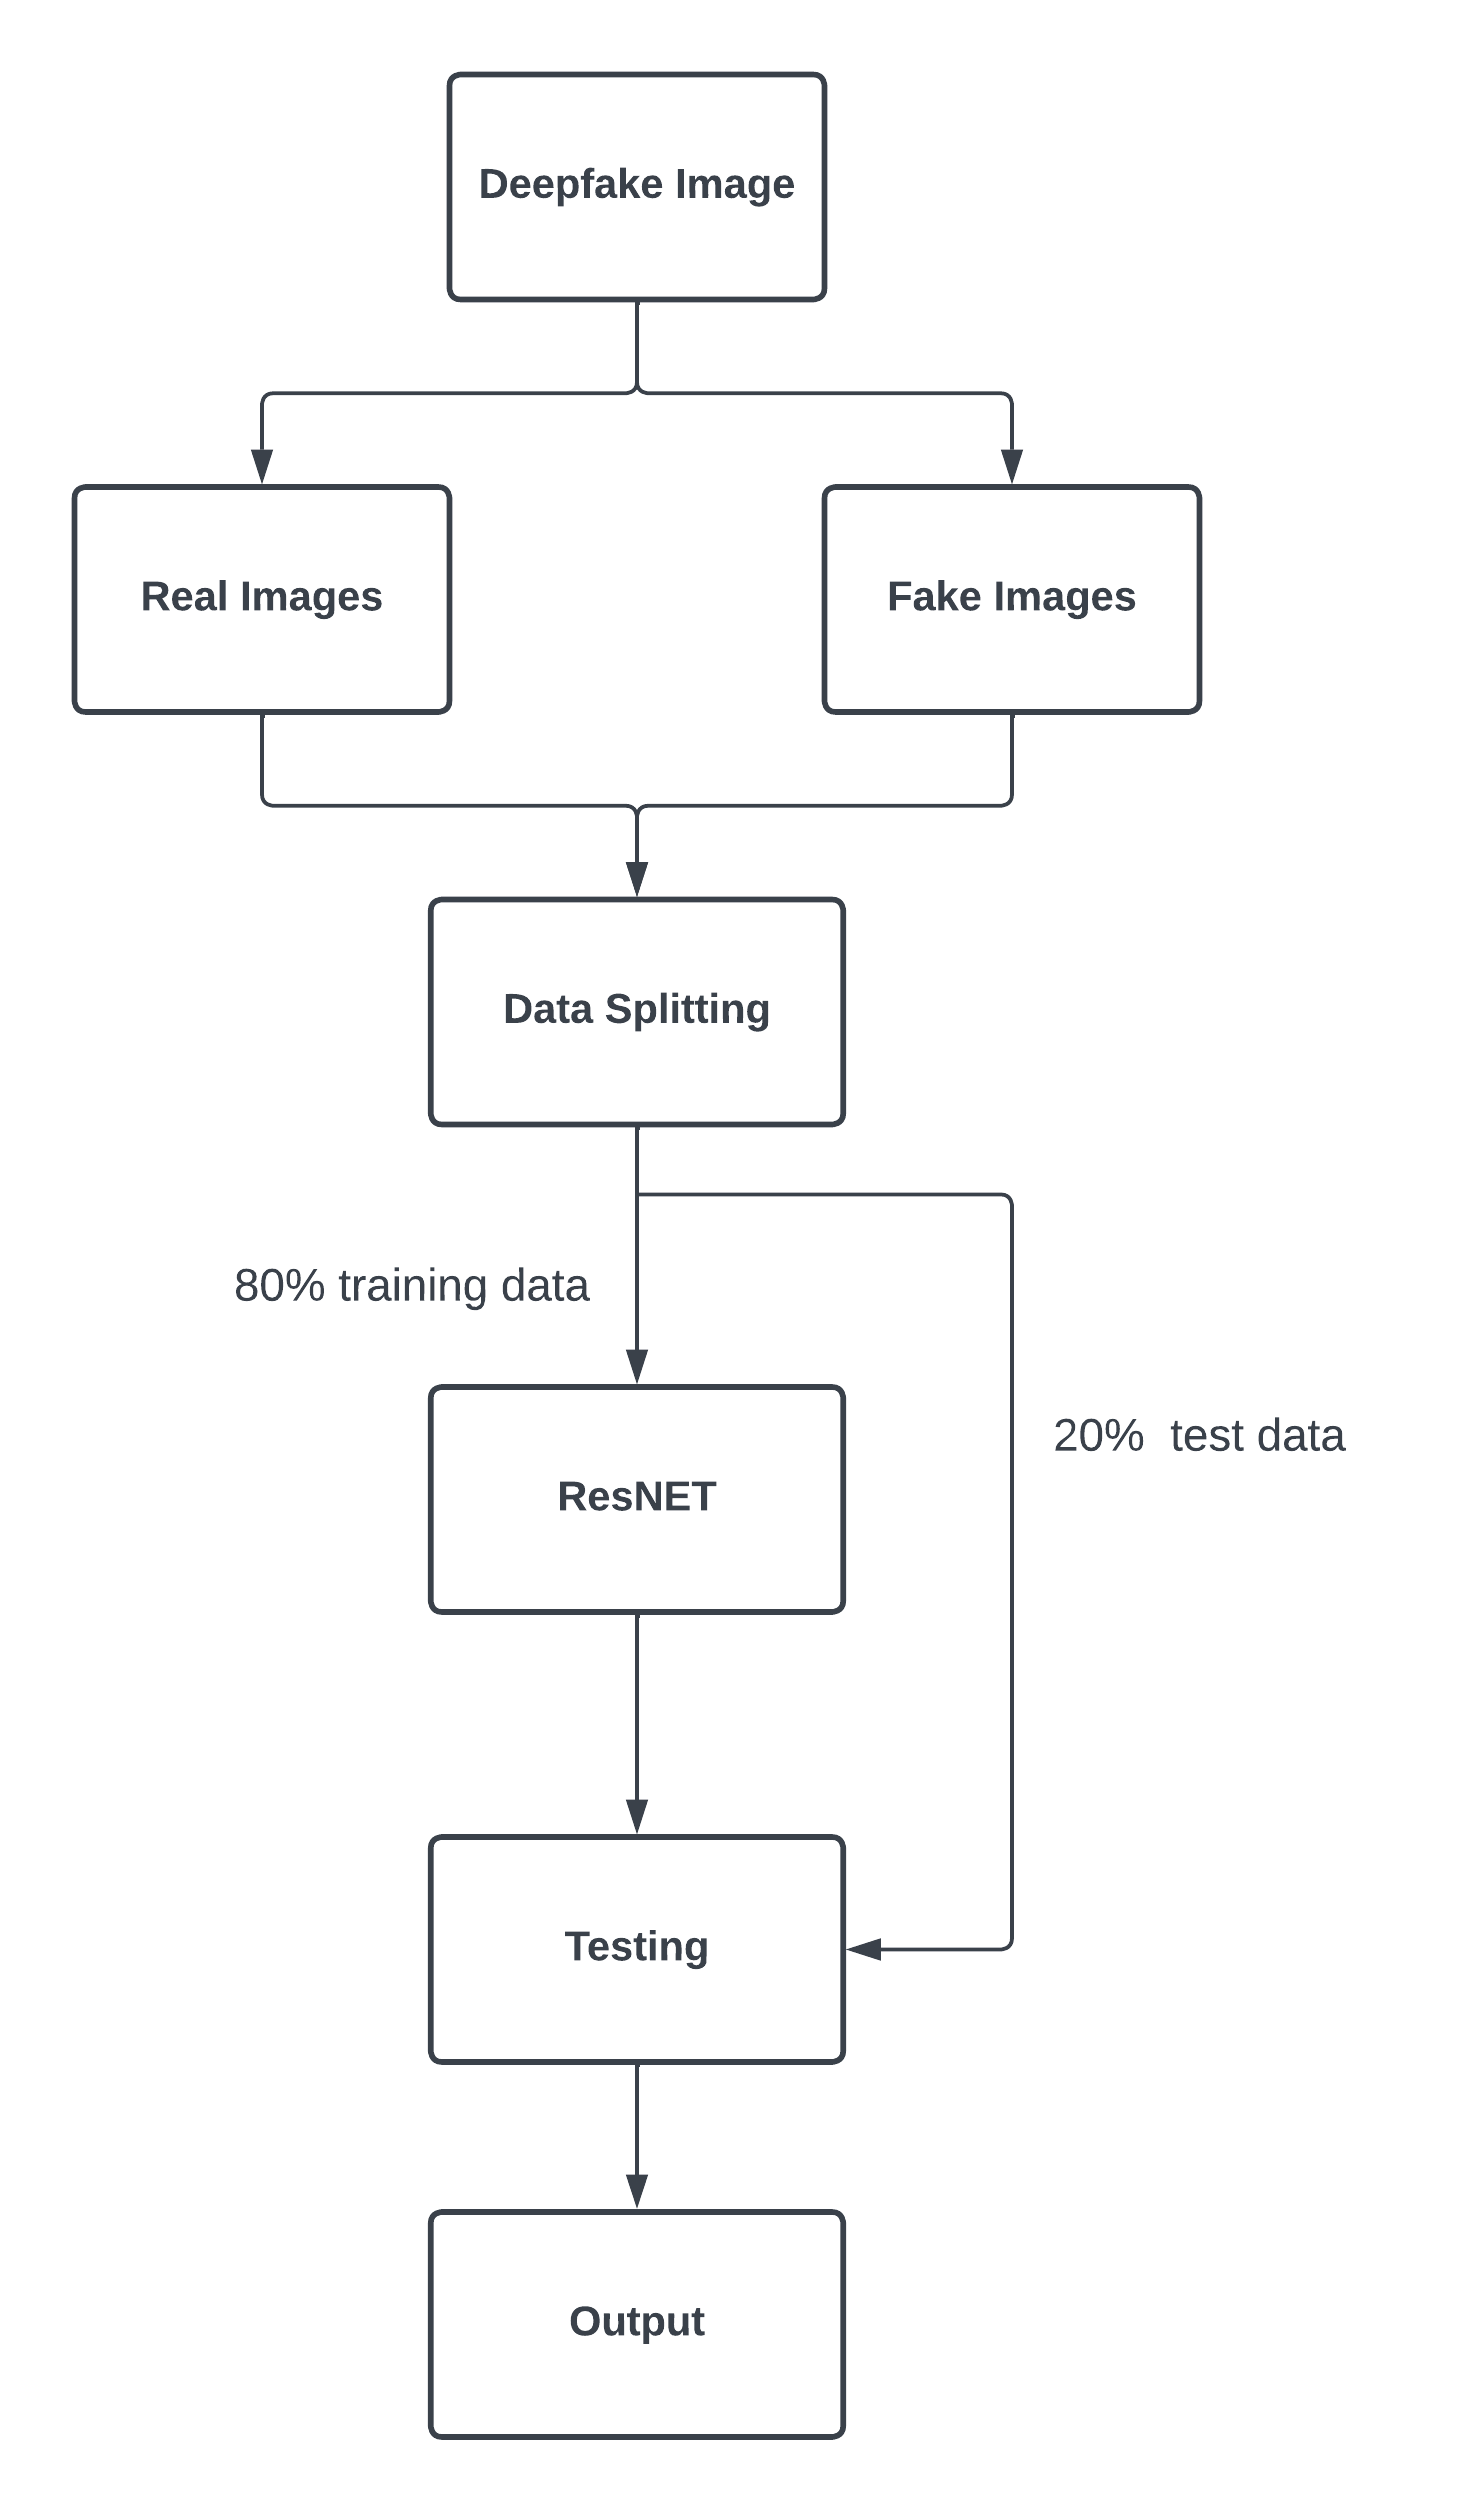
\includegraphics[width=0.25 \textheight]{./img/Block Diagram.png}
                \caption{Methodological Architecture of Our Proposed System}
            }
        \end{figure}

        \subsection*{ResNet}
        ResNet architecture introduced the concept called Residual Blocks. In this network, we use a technique called skip connections. The skip connection connects activations of a  layer to further layers by skipping some layers in between. This forms a residual block. Resnets are made by stacking these residual blocks together. 
        The approach behind this network is instead of layers learning the underlying mapping, we allow the network to fit the residual mapping. So, instead of say H(x), initial mapping, let the network fit,
        \center{F(x) := H(x) - x 
            which gives H(x) := F(x) + x}

        \begin{figure}[hbt!]
            \center{
                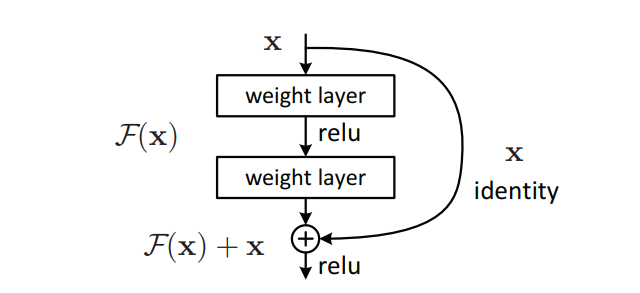
\includegraphics[width=1\textwidth]{./img/ResNet.PNG}
                \caption{ResNet}
            }
        \end{figure}


        \newpage
        \justifying
        \subsection{Gantt Chart}
            \begin{figure}[hbt!]
                \center{
                    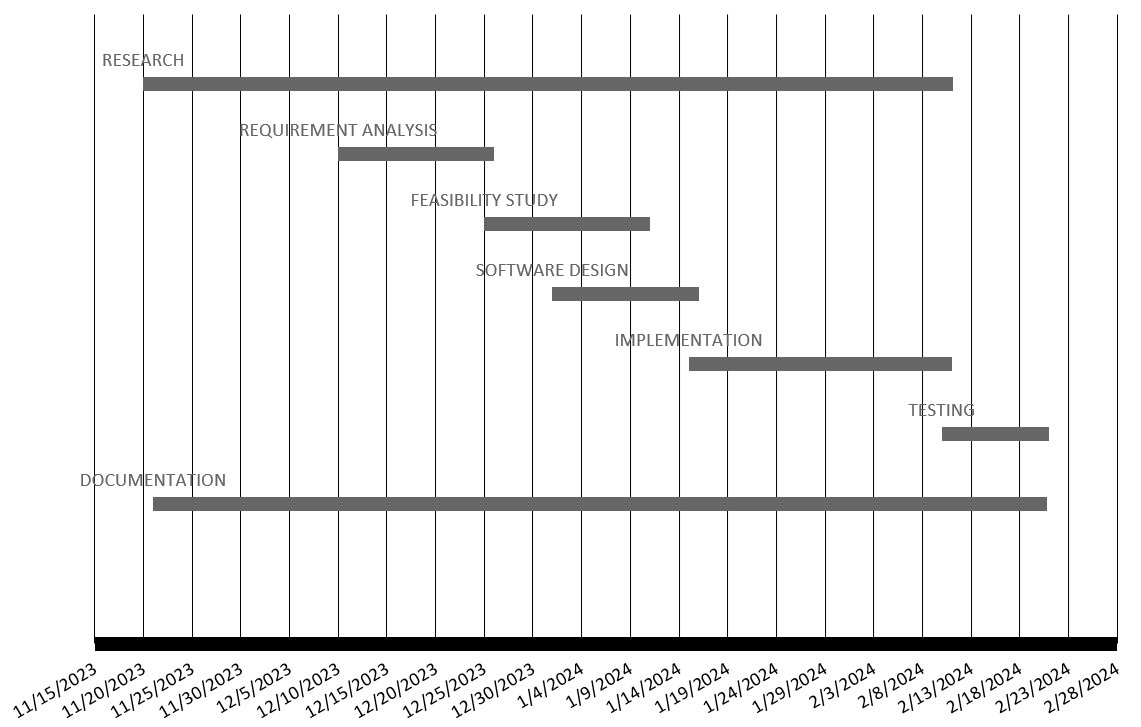
\includegraphics[width=1\textwidth]{./img/GANT_CHART.jpg}
                }
                \caption{Gantt chart}
            \end{figure}

